\documentclass[journal]{vgtc}

% TVCG Packages
\usepackage{mathptmx}
\usepackage{graphicx}
\usepackage{times}
\usepackage{multirow}
\usepackage{booktabs}
\usepackage{amsmath}
\usepackage{caption}
\usepackage{subcaption}
\usepackage[utf8]{inputenc}


% Extra Packages
\usepackage{url}
\usepackage{epstopdf}
\usepackage{arydshln} % For \hdashline in tables
\usepackage{enumitem} % For [noitemsep] in lists

% Coloring author comments
\usepackage{color}
\usepackage[usenames,dvipsnames]{xcolor}
\definecolor{Purple}{rgb}{.75,0,.85}

\newif\ifnotes
\notestrue
\newcommand{\todo}[1]{\ifnotes {\textcolor{Purple}{\bf TODO: #1\ }} \fi}

% if we want to put in page breaks to assess length
\newif\iftestbreaks
\testbreakstrue
\newcommand{\testbreak}{\iftestbreaks\newpage\fi}

% Useful abbreviations
\usepackage{xspace}
\newcommand{\etal}{\emph{et al.}\@\xspace}
\newcommand{\ie}{\emph{i.e.}\xspace}
\newcommand{\eg}{\emph{e.g.}\xspace}
\newcommand{\etals}{\mbox{\emph{et~al.}'s }}

% TODO NSF CRI / Gleicher commands
\def\naive{na\"{\i}ve}
\def\naively{na\"{\i}vely}

% Droid Sans font
%\usepackage[defaultsans]{droidsans}
%\renewcommand*\familydefault{\sfdefault} %% Only if the base font of the document is to be typewriter style
%\usepackage[T1]{fontenc}
%\linespread{1.1}

\newcommand\multipleViews{

\begin{figure}
  \centering
  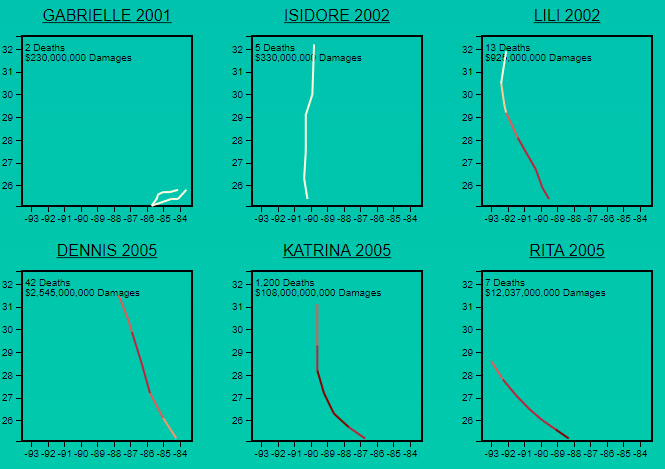
\includegraphics[width=\columnwidth]{img/brushLineGraphs}
  \caption{
    Filtered multiple views of individual hurricanes in a specified area from the brush in the animation.
  }
  \label{fig:protein-validate}
\end{figure}

}

\newcommand\brush{

\begin{figure}
  \centering
  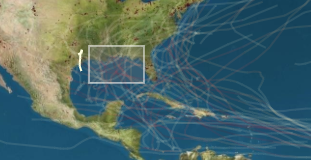
\includegraphics[width=\columnwidth]{img/brush}
  \caption{
    Brush filter in the animation.
  }
  \label{fig:protein-validate}
\end{figure}

}


\newcommand\bars{

\begin{figure}
  \centering
  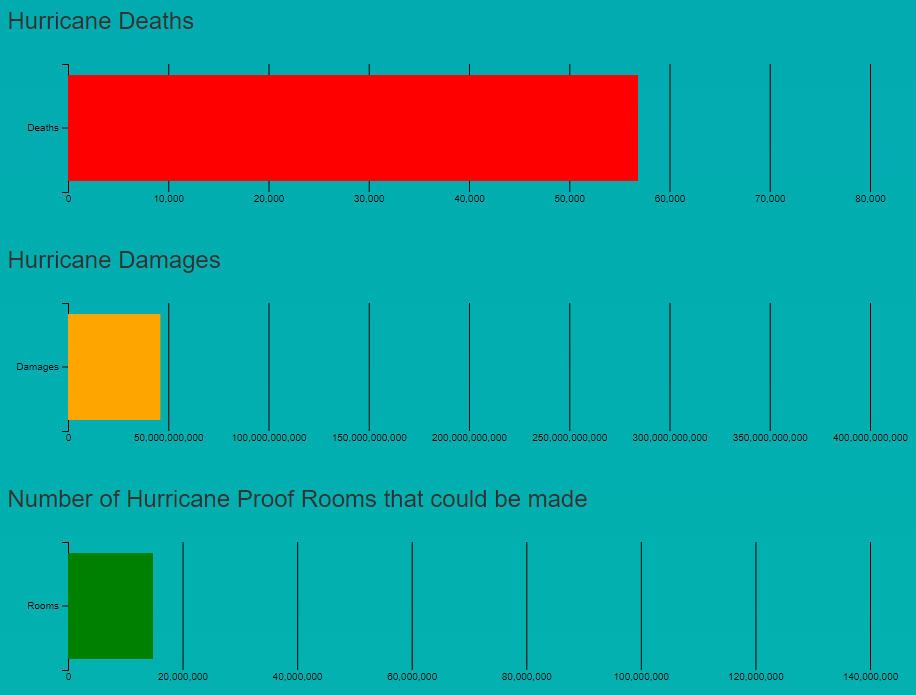
\includegraphics[width=\columnwidth]{img/bars}
  \caption{
    The three bar chars to go along with the animation to show the number of deaths accumulated, amount of damages accumulated and the number of hurricane safe houses that could be build.
  }
  \label{fig:protein-validate}
\end{figure}

}
\newcommand\testtable{

\begin{table}[]
\centering

\begin{tabular}{r c c c c}

& \multicolumn{2}{c}{Our Results} & \multicolumn{2}{c}{Their Results} \\
\multicolumn{1}{l|}{\textbf{Measures}} & \textbf{Exp} & \textbf{Control} & \textbf{Control} & \textbf{Exp} \\ \hline
\multicolumn{1}{l|}{measure A}  & 54.8  & 48.6  & 44  & 33  \\ 
\multicolumn{1}{l|}{measure B}  & 32.2  & 28.8  & 8   & 6   \\ \hdashline
\multicolumn{1}{l|}{measure C} 	& 22.8  & 19.8  & 35  & 26  \\ 

\end{tabular}

\caption{As you can see, we are the best.}
\label{tab:results}
\end{table}

}


\usepackage[bookmarks,backref=true,linkcolor=black]{hyperref} %,colorlinks
\hypersetup{
  pdfauthor = {},
  pdftitle = {},
  pdfsubject = {},
  pdfkeywords = {},
  colorlinks=true,
  linkcolor= black,
  citecolor= black,
  pageanchor=true,
  urlcolor = blue,
  plainpages = false,
  linktocpage
}

%% If you are submitting a paper to a conference for review with a double
%% blind reviewing process, please replace the value ``0'' below with your
%% OnlineID. Otherwise, you may safely leave it at ``0''.
\onlineid{0}

%% declare the category of your paper, only shown in review mode
\vgtccategory{Exploration}

\vgtcinsertpkg


\title{Ignorance of Hurricanes}

\author{Jason Abel}
\authorfooter{
\item
 Jason Abel is with Worcester Polytechnic Institute. E-mail: jabel@wpi.edu

}

%other entries to be set up for journal
% \shortauthortitle{Author \MakeLowercase{\textit{et al.}}: Title}



%% Abstract section.
\abstract{
The objective of this paper is to inform people of the dangers of hurricanes through a story animation. Over the years many people have died to hurricanes and there has been lots of damages. This paper takes a look at hurricane paths, death count, damage count, and evacuation types of large scale hurricanes in the Atlantic ocean. From the information gathered, it was concluded that people may underestimate hurricanes and may not prepare for hurricanes well enough due to the large amounts of death and damages accumulated over time. It is important to note that the number of deaths has significantly reduced over the years however the amount of damages has increase significantly as well. It is estimated that if we took all the money accumulated in damages, we could produce over 120 million hurricane proof rooms. The main message that this story animation is that people should prepare for hurricanes much more and to not underestimate hurricanes. This paper aims to get people to understand that hurricanes are unpredictable. This paper will talk about the background of hurricane related information as well as the methodology of how this animation was created in order to tell the story about hurricanes ignorance. Finally, the results found were stated and discussed along with a final conclusion made about the project.
} 

\keywords{Hurricanes, Visualization, Animation, Story, Information}

%% ACM Computing Classification System (CCS). 
%% See <http://www.acm.org/class/1998/> for details.
%% The ``\CCScat'' command takes four arguments.

% \CCScatlist{ % not used in journal version
%  \CCScat{K.6.1}{Management of Computing and Information Systems}%
% {Project and People Management}{Life Cycle};
%  \CCScat{K.7.m}{The Computing Profession}{Miscellaneous}{Ethics}
% }

%% Uncomment below to include a teaser figure.
% Teaser should be jnds for -pcp versus +pcp (distinguishable; not distinguishable; target; not distinguishable; distinguishable)
\teaser{
  \centering
  
\includegraphics[width=\textwidth]{img/teaser}
  \caption{Hurricane animation currently displaying Hurricane Andrew}
  \label{fig:teaser}
}

%% Uncomment below to disable the manuscript note
%\renewcommand{\manuscriptnotetxt}{}

%% Copyright space is enabled by default as required by guidelines.
%% It is disabled by the 'review' option or via the following command:
% \nocopyrightspace

%%%%%%%%%%%%%%%%%%%%%%%%%%%%%%%%%%%%%%%%%%%%%%%%%%%%%%%%%%%%%%%%
%%%%%%%%%%%%%%%%%%%%%% START OF THE PAPER %%%%%%%%%%%%%%%%%%%%%%
%%%%%%%%%%%%%%%%%%%%%%%%%%%%%%%%%%%%%%%%%%%%%%%%%%%%%%%%%%%%%%%%%

\begin{document}

%% The ``\maketitle'' command must be the first command after the
%% ``\begin{document}'' command. It prepares and prints the title block.

%% the only exception to this rule is the \firstsection command
\firstsection{Introduction}

\maketitle

%% \section{Introduction} %for journal use above \firstsection{..} instead

% Introduction section is automatically added
As a major public transportation, airline market has been ushering a booming development. On a global scale, a continuous world-wide growth of air traffic could be observed, and according to several market researches, the growth is expected to maintain positive rates up to 2030.

However, there are many factors that affect the performance of the commercial aviation system, which can lead to annoying results to their passengers sometimes. Given the uncertain factors of the whole aviation system, passengers usually have to plan their travel many days or even months before the departure date. Meanwhile, in order to decrease the trip costs, avoid the rush traffic hours, and then obtain a relaxed travel experience, travelers also hope to gain as more detailed information as possible.

Converting the traditional numeric information into a more vivid visualization form, could help the viewers gain their desired information efficiently and easily. So we intend to build a map based interactive consulting visualization, which combines two date sets coming from the US Department of Transportation Bureau of Transportation Statistics. We hope this application can reveal some potential patterns under the flight records and display them to the viewers.

We apply D3.js library to build the whole data visualization including one map view which is used to depict the airports and the airlines. While users move the mouse over an area belonged to a specific state, the area will highlight of which the color change and the name of that state will pop up. Once users click the state, it will filter out other states, that only displays the airports sited inside the chosen state. For sure, we also provide a button placed at the top middle of the web page, to reset the map view to its original status. Correspondingly, the right-side bar chart will change once users click a specific state. The bar chart we use here is to display a comparison of fight delay period among at most six airline companies. This bar chart is a variety of the plain bar, which is divided horizontally into upper and lower part, each of them present the degree of departure and arrival delay respectively. Initially, this stack bar chart will display average delay time across all the flight data. Of course, to make the bar chart more practical, we also append the numeric value of the flight delay time while users move the mouse over a specific part of the bar chart.\cite{heiberger2014design} Meanwhile, the word cloud view will change as a reaction of the click action on the stack bar chart, the key words it shows every time will change correspond with the content of passengers’ tweets. Most of the words are the reflection of the feel of the passengers, either is positive or negative.



%\S\ref{sec:conclusion}.

\testfigure

%\testtable

\section{Background}
As the time goes by, the use of coordinated multiple views has been changing and expanding a lot, in addition it also becomes part of larger sense making environments where the techniques are being used to analyze large datasets, integrate alternate viewpoints, and generate nuggets of information.\cite{roberts2007state} Nowadays, D3.js library is one of the most popular tools to implement the coordinated multiple views and then analysis large data set. It is worth and quite practical to apply these ideas and tools while building the final project. Meanwhile, data visualization is not just a way that simply transforms the data into several tables or charts, instead, it also involves pre-processing on data such as clearing, filtering, mapping or other aggregation operation. The process that chose appropriate visualization pattern with the dataset is challenging, but on the other hand, a good vis always provides its audiences an intuitive and logical experience. Utilizing all the handy techniques we have to develop an extension of the previous project, is a good study path for our future work.

There are three important parts: designing the whole visualization, fixing the big data problem (our original dataset contains 300M+ rows), achieving the interactions between visualizations with the help of d3 and react instead of using dispatch.

\section{Method}

Basically we used D3.js to build each data visualization including US Map, Stacked Bar Chart, Word Cloud. 

\subsection{Interaction}
People usually use dispatch which is a tool to create interaction between data visualization views to create interactions, but we decide to use React.js to do the same thing instead of dispatch.

React is a JavaScript library for building user interfaces, the core idea behind it is integrating separate parts into a whole thing (class) and controlling each part's state. For example, we can create a simple spinning button by combining a button element, a spinning figure, and a state variable to control spinning or not. We embed the three things into a class SpinningButton, we set the spinning state with false as default, when user click the button, setting the state with true, showing the spinning figure and starting up a timer function as the same time, when time running out, set the state with false back, hidden the spinning figure. 

As you can see, we can use this kind of idea to control our visualization information and transport the information by react states, the figure~\ref{fig:stateEx} shows our state. 
\stateEx



\subsection{Big Data Problem}

As we mentioned before, our original dataset contains 300M+ rows, the data size is above 600MB, it is definitely not a good idea to store the data along with the website. Instead of uploading the dataset, we create a MongoDB (a NoSQL database) database to store our data. There are two reasons we choose MongoDB\cite{boicea2012mongodb}, the first reason is it is NoSQL data structure as JSON format, it's convenient to I/O data. It has a good compatible with Amazon Website Service which is also good for transporting data. Of course, MongoDB is also good for aggregation operation which help us to retrieve different kind of query combinations. \cite{keim2013big}

Amazon Website Service could help us to build our APIs to retrieve MongoDB data in cloud, it has a high computing performance and compatible with MongoDB\cite{jackson2010performance}.

With the help of MongoDB and AWS, we don't need to uploading the whole large dataset which could make the website run slowly. On the other hand, we can keep the whole dataset without any pruning and modification which could lead information loss.

We can see in figure~\ref{fig:mongoEx}, our flights collection is up to 1.2G which is super large.
\mongodbEx

\subsection{D3 Transition}
When the data changes in a d3 views, what is the interesting thing we may notice? That is transition. It's boring if a data visualization just change their view by refreshing the whole view, that is deleting the whole dataset, and replacing with new dataset. D3 provides a really good way to deal with this problem, it's called, enter, update and exit as shown in figure~\ref{fig:transition}. It's super useful and interesting part of D3.js and also it's hard to understand, as lease we spent a lot of time to understand these kind of concepts. Generally, the processes are, supposing our view has been implemented. Now, we need to update the view by the new dataset. First, the D3 collects the previous dataset and new coming dataset, and secondly, the D3 finds the common part and different part (we could or we better specify which data field we are going to compare ), and lastly, the D3 update the different part and remove the useless data. From these procedures, we could efficiently and perfectly control the transitions.\cite{buja1991interactive}  
\transition

\subsection{Word Cloud}
\wordcloud
Word Cloud is a powerful tool for sentiment analyzing\cite{heimerl2014word}. We firstly tried to tokenize Tweeter user's whole text and count each word's frequency for showing in the word cloud. But it turns out not a good choice since there are so many stop words and useless characters, even though we preprocessed the user's text, eliminate all possible stops words and special characters\cite{miner2012practical}, our results are not as good as what we think (see in figure~\ref{fig:badwordcloud}). Thus we choose an alternate way to present user attitude, that is extract all emoji characters! We can see although it's not good enough, we can still tell the overall attitude from this emoji word cloud (see in figure~\ref{fig:wordcloud}).
\badwordcloud
\section{Results}
With the help of D3.js, React.js, MongoDB and Amazon Website Service, we successfully create our whole interactive data visualization. Our visualization shows the average airline departure delay time, the average airline arrival delay time and Tweeter user's sentiment. User could click any state to show the information corresponding the all airports in this specific state. User also could click the stack bar chart to show each specific airline's corresponding information. 

\section{Other Useful articles Influence us}
It gives an idea that how to depict a visualization of adjacency relations in hierarchical data, especially with a huge dataset. \cite{holten2006hierarchical}

They presented a visual analysis of Twitter time-series, which combines sentiment and stream analysis with geoand time-based interactive visualizations for the exploration of real-world Twitter data streams. \cite{hao2011visual}

It introduced a novel visualization called NodeTrix.\cite{henry2007nodetrix} 

This paper mainly introduces how and why the authors visualize cyber security session data by an interactive behavior map. They encoded an action as city and user sessions as trajectories going through the cities. They illustrated how they explore relationships between actions, identity patterns of the typical session and detect anomaly behaviors.\cite{de2003visual}

The D3.js library has become a super popular tool for developing visualization on the website. More and more people use this kind of technology to improve their website outlook as well as the actual needs. However, it is time-consuming when people only want to change their visualization's appearance. This article tells how to use a pair of tools for deconstructing and restyling existing D3 visualization without understanding the underlying code and logic.\cite{harper2014deconstructing}

This article presents their approach to combine sentiment analysis with a new term association technique as well as a geo-temporal visualization for an effective analysis of large customer feedback streams. They introduce a feature and geo-based stream analysis technique that automatically detects which attributes (features) are frequently commented on, which attributes have interesting sentiments patterns, which attributes cluster significantly in certain geo-locations, and what terms often occur together. They also introduce two new geo-temporal visualizations (pixel sentiment and key term geo maps) that help users analyze large volumes of web surveys and Twitter data.\cite{hao2013visual}

Nowadays data visualization exists in everywhere our lives. We can see data visualization in newspaper, TV, Internet, conmmercial advertisements, etc. With the widely use of data visualization, there is a growing awareness of the uncertainty problem within the visualization community, and many traditional techniques are being extended to represent not only the data, but also the uncertainty information associated with the data. We call this visualization of uncertainty. In addition, it is important to realise that, even if there is certainty about the data, errors can occur in the process of turning the data into a picture. We call this uncertainty of visualization. This paper aims to review the current state of the art in uncertainty in scientific visualization, looking at both of these aspects.\cite{brodlie2012review}

Automatic exploration of semantic classification of ducuments is becoming more and more popular, there are many tasks measuring the documents or chunks of text such as automatic sentiment analysis, which measures the text based on emotive categories such as positive and negative. However, there is limited progress on how to visualize the affective content of documents and describes an interactive capability for exploring emotion in a large document collection.

This paper described an approach of how these measurements might be presented to the users for exploration and added value. This approach includes identifying the affective content of documents, as well as possible ways of visualizing it and presenting those results analytically.\cite{gregory2006user}




\subsection{Conclusion}
\label{sec:conclusion}
This paper is mainly trying to find a way to create a interactive visualization by combining React.js and D3.js. The visualization is also helpful for people who want to know what is the average delay of each airlines and what is the people's attitude by presenting Tweeter's sentiment information. 

It also find a way to deal with big data problem when the dataset it's too large to upload to website. 

Moreover, it gives a good example to use D3 transition for improving the visualization's quality.

At the end, we find that combining React and D3 is a good way to develop interactive visualization, it's efficient, easy to control and extensible. Although our current visualization's interaction is not fast, that is because the transporting problem between the AWS and MongoDB (it may be resulted by some bad query sentences), and the dataset is too large to do complicate query operation like finding all given airline in some airports. That is nothing to do with the React and D3.

In the future, we could add more views to allow user to discover more information. For example, we could add a timeline to find the delay information according the time range. We also could add a functionality that user could click any two of airports to see the corresponding information between the two airports, or click any two of us states to show corresponding information. Furthermore, we could find a more efficient and useful way to preprocess Tweeter User's tweet and present them in Word Cloud.




%% if specified like this the section will be committed in review mode
\acknowledgments{
The Author would like to acknowledge Lane Harrison for his insight in helping come up with ideas on how to build the visualization and the guidance provided throughout the project. 
}

\bibliographystyle{abbrv}
\bibliography{paper.bib}


\end{document}